\subsection{Парабола}

\textsl{Парабола} --- геометрическое место точек, равноудалённых от данной прямой (называемой \textit{директрисой} параболы) и данной точки (называемой \textit{фокусом} параболы).

Каноническое уравнение параболы имеет следующий вид:
\begin{equation}
y^2=2px
\end{equation}
Где $p$ --- \textit{фокальный параметр}, равный расстоянию между фокусом параболы и директрисой или удвоенному расстоянию между фокусом параболы и вершиной.

Парабола в полярной системе координат $(\rho,\varphi)$ с центром в фокусе и нулевым направлением вдоль оси параболы (от фокуса к вершине) может быть представлена в виде следующего уравнения:
\begin{equation}
\rho(1+\cos\varphi)=p
\end{equation}

Эксцентриситет параболы равен $e=1$.
Так как парабола не является замкнутой $\Rightarrow$ она не имеет \textit{большой} и \textit{малой полуоси}.

Ниже представлено \textit{оптическое свойство} параболы:

Пучок лучей, параллельных оси параболы, отражаясь в параболе, собирается в её фокусе. И наоборот, свет от источника, находящегося в фокусе, отражается параболой в пучок параллельных её оси лучей.
\begin{figure}[h!]
\centering
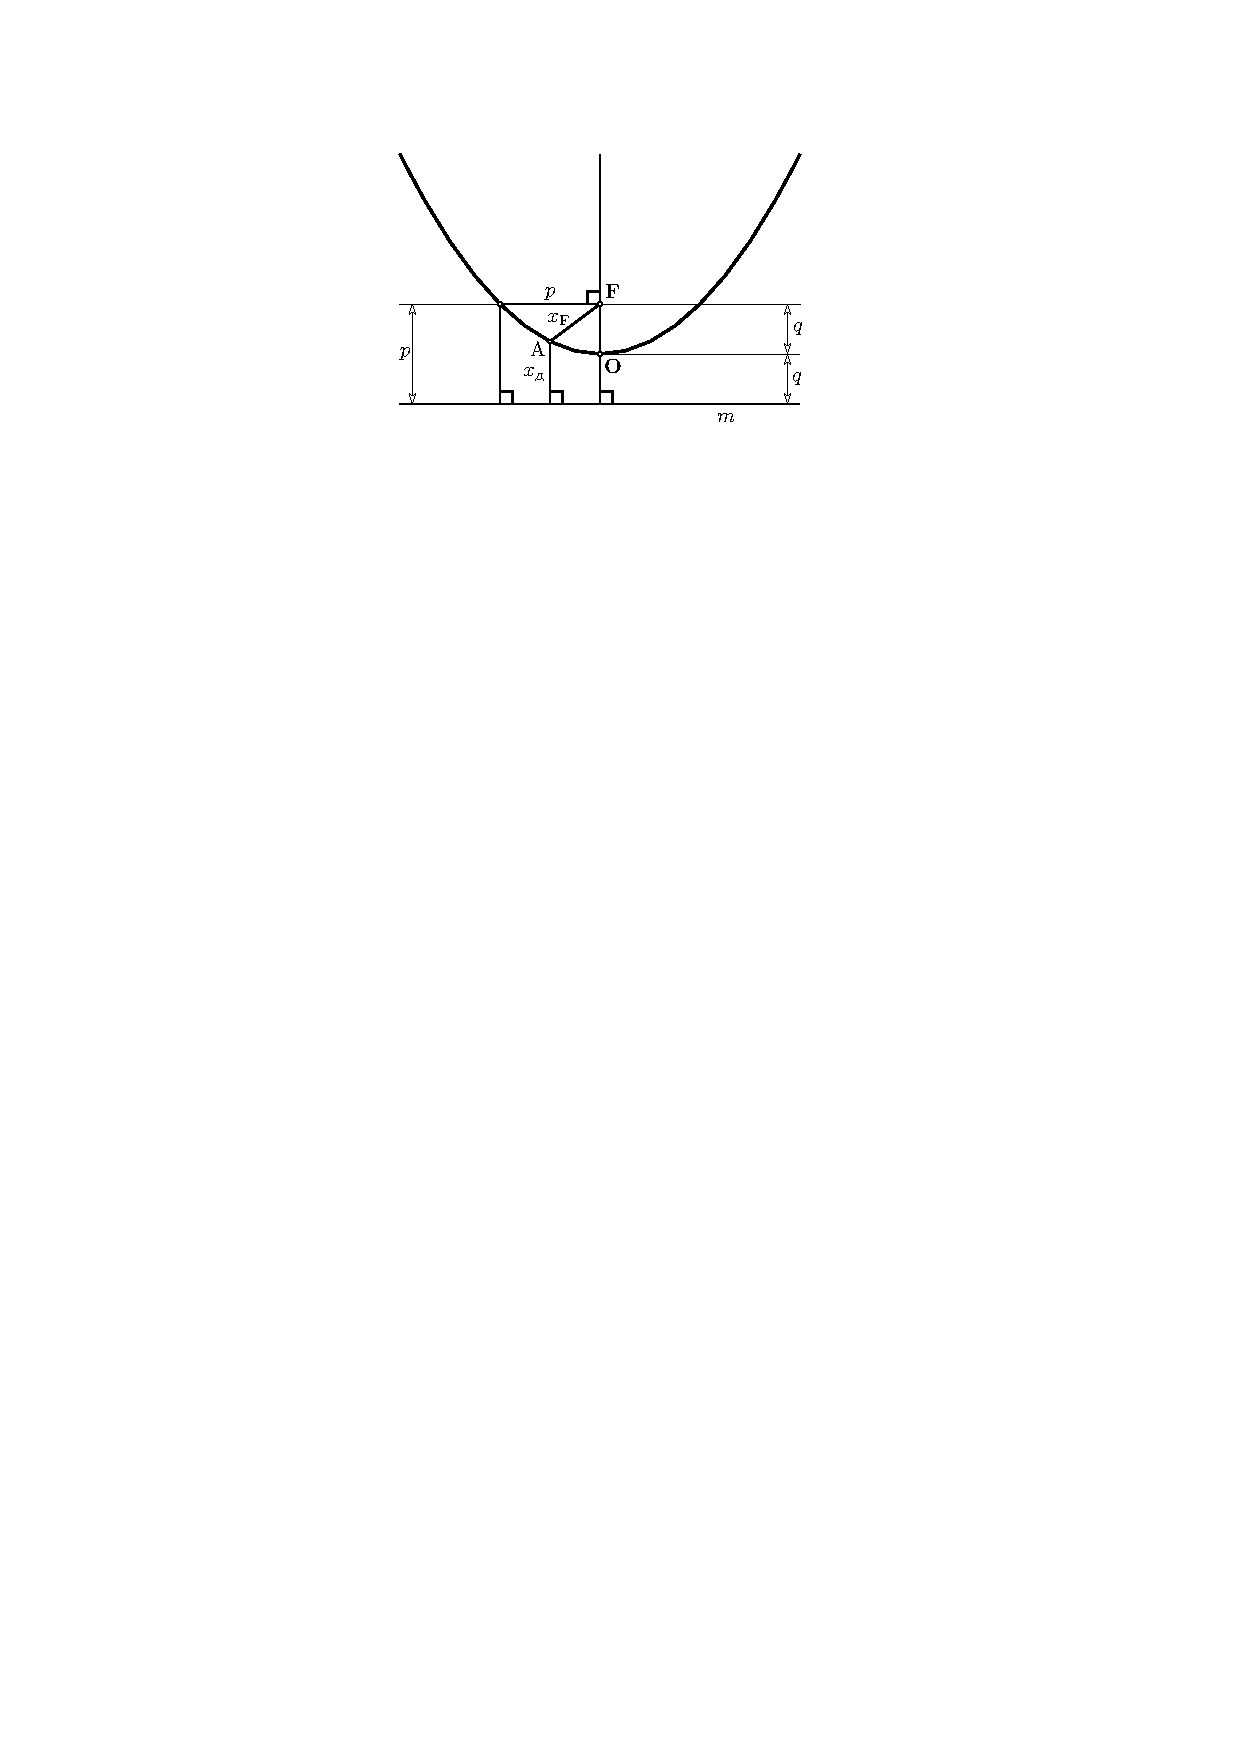
\includegraphics[width = 0.8\textwidth]{Parabola}
\caption{Парабола \label{pic:the-pic}}
\end{figure}
